\documentclass[journal,12pt,twocolumn]{IEEEtran}
\usepackage{graphicx}
\graphicspath{{./images/}}
\usepackage{amsmath,amssymb,amsfonts,amsthm}
\newcommand{\myvec}[1]{\ensuremath{\begin{pmatrix}#1\end{pmatrix}}}
\usepackage{listings}
\usepackage{watermark}
\usepackage{titlesec}
\let\vec\mathbf
\lstset{
frame=single, 
breaklines=true,
columns=fullflexible
}
\thiswatermark{\centering \put(0,-105.0){
\includegraphics[scale=0.2]{logo2.png}} }
\title{\mytitle}
\title
{
Matrix Assignment - Circle
}
\author{Surajit Sarkar}
\begin{document}
\maketitle
\tableofcontents
\bigskip


\section{\textbf{Problem}}
Consider a family of circles passing through two fixed points A(3,7) and B(6,5) show that the chords in which the circle $x^2+y^2-4x-6y-3=0$ cuts the members of the family are concurrent at a point.Find the coordinates of this point ?
\section{\textbf{solution}}


\begin{equation}
    \vec{x^2+y^2}-9{\vec x}-12{\vec y}+53=0
\end{equation}
\begin{equation}
    {\vec{{x}}^T{\vec V}_1{\vec x}+2{\vec u}_1^T{\vec x}}+f_1
\end{equation}
\begin{equation}
    \vec{x}^T{\myvec{1&0\\0&1}}{\vec {x}+2 {\myvec{{\frac{-9}{2}}-6} {\vec {x }}}}+ 53=0
\end{equation}

Where
\begin{equation}
    \vec{V_1}={\myvec{1&0\\0&1} }
\end{equation}
\begin{equation}
    \vec{u_1}={\myvec{{\frac{-9}{2}}-6}}
\end{equation}
\begin{equation}
    f_1=53
\end{equation}
Equation of circle with A and B as diameter\\
Equation of line passing through A and B
\\ 
\\Direction vector  
  
\begin{equation}
    \vec{m= A-B}
\end{equation}
\\Normal vector

\begin{equation}
    \vec{n} = \vec{R}_{\frac{\pi}{2}} \myvec{\Vec{m}}
\end{equation}
where
    \[ \vec{R}_{\frac{\pi}{2}} = \myvec{\cos  \theta & -\sin \theta \\ \sin \theta & \cos \theta}\]
Equation of $L_1$
\begin{equation}
    \vec{n}^T{\myvec{\vec x-\vec A}}=0
\end{equation}
\begin{equation}
    \vec {n^T x}-\vec {n^TA}=0
\end{equation}
Given circle
\begin{equation}
    \vec{{x}^2+{y}^2}-4{\vec x}-6{\vec y}-3=0
\end{equation}
\begin{equation}
    {\vec{{x}}^T{\vec V}_2{\vec x}+2{\vec u}_2^T{\vec x}}+f_2
\end{equation}
\begin{equation}
   { \vec{{x}}^T{\myvec{1&0\\0&1}}{\vec x}}+2{\myvec{-2&-3}}{\vec x}-3=0
\end{equation}
Where
\begin{equation}
    {\vec V}_2 = {\myvec{1&0\\0&1}}
\end{equation}
\begin{equation}
    {\vec{u}_2}={\myvec{-2&-3}}
\end{equation}
\begin{equation}
    f_2={-3}
\end{equation}
Common chord is given by
\begin{equation}
    {\vec{c}_1-{\vec c}}_2+\lambda{L_1}
\end{equation}

Where\\ $c_1$ is circle having A and B as diameter\\
        $c_2$ is given circle


\begin{equation}
    \vec{\myvec{-5-6}}{\vec x}+56+\lambda L_1
\end{equation}
\begin{equation}
    \vec{\myvec{5&6}}{\vec x}=56  ---\myvec{L_2}
\end{equation}
Using python we get the $L_1$ and intersection point
\begin{equation}
    \vec{\myvec{2&3}}{\vec x}=27 ---\myvec{L_1}
\end{equation}
\begin{equation}
    \vec{\myvec{5&6\\2&3}}{\vec x}={\myvec{56\\27}}
\end{equation}
%\begin{equation}
%    \vec {A x= b}
%\end{equation}
%\begin{equation}
%    {\vec{x={A}}^{-1} {\vec b}}
%\end{equation}
\begin{equation}
    \vec{x}={\myvec{2,7.667}}
\end{equation}
\begin{lstlisting}
https://github.com/sssurajit/fwc/blob/main/matrix/circle/codes/scircle.py
\end{lstlisting}

\section{\textbf{Figure}}

    \centering
    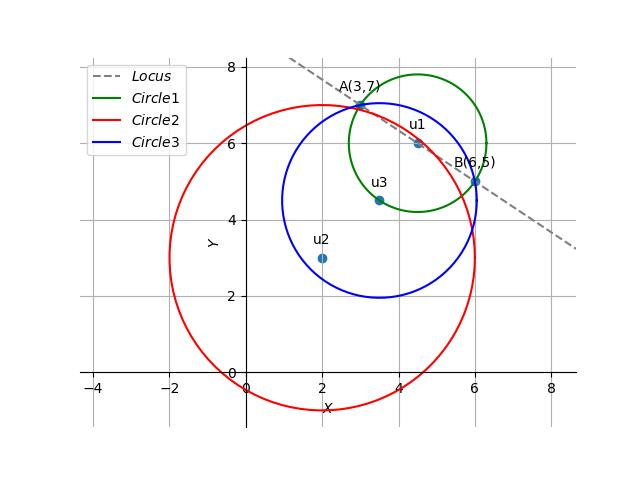
\includegraphics[width=\columnwidth]{fig.jpg}
    \label{fig:my_label}
    
\section{\textbf{Code Link}}

\begin{lstlisting}
https://github.com/sssurajit/fwc/blob/main/matrix/circle/codes/circle.py
\end{lstlisting}
Execute the code by using the command
\\ \textbf{python3 circle.py}

\end{document}
